\documentclass{homework}

\usepackage{graphicx}
\usepackage{subfig}
\usepackage{siunitx}
\usepackage{subcaption}
\usepackage{amsmath}
\usepackage{bbm}

\captionsetup{compatibility=false}

\title{Homework}
\author{Daniel Kadyrov}

\Title{Homework \#1}
\DueDate{February 11th, 2020}
\ClassName{Machine Learning}
\ClassNumber{CS559WS}
\ClassSection{Spring 2020}
\Instructor{Professor In Suk Jang}
\Author{Daniel Kadyrov}
\AuthorID{10455680}

\begin{document}

\maketitle

\begin{problem}[1]
    By using a change of variables, verify that the univariate Gaussian distribution given by:

    $$
    N(x \mid \mu , \sigma^2) = \frac{1}{\sqrt{2\pi\sigma^2}}\exp\{
        -\frac{1}{2\sigma^2}(x-\mu)^2
        \}
    $$

    satisfies $E(x) = \mu$. Next, by differentiating both sides of normalization condition

    $$
    \int_{-\infty}^{-\infty}N(x \mid \mu, \sigma^2) dx = 1
    $$

    with respect to $\sigma^2$, verify that the Gaussian satisfies $E(x^2)=\mu^2+\sigma^2$.
\end{problem}

\begin{solution}
    $$
    E(x) = \int_{-\infty}^{\infty} p(x|\mu, \sigma^2)x dx = E(x) = \int_{-\infty}^{\infty} \frac{x}{\sigma\sqrt{2\pi}}\exp\left\{-\frac{(x-\mu)^2}{2\sigma^2}\right\} dx
    $$
    $$
    E(x) = \int_{-\infty}^{\infty} \frac{x-\mu}{\sigma\sqrt{2\pi}}\exp\left\{-\frac{x^2}{2\sigma^2}\right\} dx = 
    \int_{-\infty}^{\infty} \frac{x}{\sigma\sqrt{2\pi}}\exp\{-\frac{x^2}{2\sigma^2}\} dx -
    \int_{-\infty}^{\infty} \frac{\mu}{\sigma\sqrt{2\pi}}\exp\{-\frac{x^2}{2\sigma^2}\} dx
    $$

    The first part of the integral: 

    $$ 
    -\int_{0}^{-\infty}x\frac{1}{\sigma\sqrt{2\pi}}\exp\left\{-\frac{x^2}{2\sigma^2}\right\}dx + \int_{0}^{\infty}x\frac{1}{\sigma\sqrt{2\pi}}\exp\left\{-\frac{x^2}{2\sigma^2}\right\}dx = 
    $$
    $$\int_{0}^{\infty}(-x)\frac{1}{\sigma\sqrt{2\pi}}\exp\left\{-\frac{(-x)^2}{2\sigma^2}\right\}dx + \int_{0}^{\infty}x\frac{1}{\sigma\sqrt{2\pi}}\exp\left\{-\frac{x^2}{2\sigma^2}\right\}dx =
    $$
    $$
    -\int_{0}^{\infty}x\frac{1}{\sigma\sqrt{2\pi}}\exp\left\{-\frac{x^2}{2\sigma^2}\right\}dx + \int_{0}^{\infty}x\frac{1}{\sigma\sqrt{2\pi}}\exp\left\{-\frac{x^2}{2\sigma^2}\right\}dx = 0
    $$

    So now the integral is: 

    $$
    E(x) = \int_{-\infty}^{\infty}\mu\frac{1}{\sigma\sqrt{2\pi}}\exp\left\{-\frac{x^2}{2\sigma^2}\right\} dx = \frac{2\mu}{\sqrt{\pi}}\int_0^\infty e^{-x^2} dx
    $$

    $$
    E(x) = \lim_{i \to \infty} \frac{2\mu}{\sqrt{\pi}} \int_0^i e^{-x^2} dx  = \mu \lim_{i \to \infty} \text{erf}(i) = \mu \Leftarrow
    $$

    $$
    E(x)=\mu \rightarrow E(x)^2 = \mu^2
    $$

    $$ 
    E(x^2) - E(x)^2 = E(x^2) - \mu^2 = \sigma^2
    $$

    $$ 
    E(x^2) = \mu^2 + \sigma^2 \Leftarrow
    $$


\end{solution}

\newpage
\begin{problem}[2]
    Use $E(x) = \mu$ to prove $E(xx^T)=\mu\mu^T+\Sigma$. Now, using the results two definitions, show that:
    
    $$
    E[x_n x_m] = \mu\mu^T + I_{nm}\Sigma
    $$

    where $x_n$ denotes a data point same from a Gaussian distribution with mean $\mu$ and covariance $\Sigma$,and $I_{nm}$ denotes the $(n,m)$ element of the identity matrix. Hence prove the result (2.124)
\end{problem}

\begin{solution}
    \begin{equation*}
        \begin{split}
            \Sigma   & = E[(x-E[x])(x-E[x])^T ] \\
                & = E[xx^T-xE[x]^T - E[x]x^T + E[x]E[x]^T] \\
                & = E[xx^T - x\mu^T -\mux^T +\mu\mu^T] \\
                & = E[xx^T] - \mu\mu^T -\mu\mu^T + \mu\mu^T \\
                & = E[xx^T] - \mu\mu^T
        \end{split}
    \end{equation*}
    \begin{equation*}
        E[xx^T] = \mu\mu^T + \Sigma \Leftarrow
    \end{equation*}

    Since $I_{nm}\Sigma = \Sigma I_{nm} = \Sigma$: 

    \begin{equation*}
        E[xx^T] = \mu\mu^T+I_{nm}\Sigma \Leftarrow
    \end{equation*}
\end{solution}
\newpage
\begin{problem}[3]
    Consider a linear model of the form:

    $$
    f(x,w) = w_0 + \sum_{i=1}^D w_i x_i
    $$

    together with a sum of squares/loss function of the form:

    $$
    L_D(w) = \frac{1}{2} \sum_{n=1}^{N} (f(x_n,w)-y_n)^2
    $$

    Now suppose that Gaussian noise $\epsilon_i$ with zero mean and variance $\sigma^2$ is added independently to each of the input variables $x_i$. By making use of $E[\epsilon_i]=0$ and $E[\epsilon_i \epsilon_j]=\delta_{ij}\sigma^2$, show that minimizing $L_D$ averaged over the noise distribution is equivalent to minimizing the sum of square error for noise-free input variables with the addition of a weight-decay regularization term, in which the bias parameters $w_0$ is omitted from the regularizer.
\end{problem}

\begin{solution}
    \begin{equation*}
        y_n(x_n, w) = w_0 + \sum_{i=1}^D w_i(x_{ni}+\epsilon_{ni}) = w_0 + \sum_{i=1}^D w_i x_{ni}+\sum_{i=1}^D w_i \epsilon_{ni} = y(x_n, w) + \sum_{i=1}^D w_i
    \end{equation*}
    \begin{equation*}
        \begin{split}
    E_{dn}(w) & = \frac{1}{2} \sum_{n=1}^{N} (y_n(x_n, w) - t_n)^2 = \frac{1}{2} (y(x_n, w) + \sum_{i=1}^{D} w_d \epsilon_ni -t_n )^2 \\
            & = \frac{1}{2} \sum_{n=1}^{N} ((y(x_n, w) - t_n)^2 + 2(y(x_n, w) - t_n)(\sum_{i=1}^{D} w_d \epsilon_{ni})+ (\sum_{i=1}^D w_d \epsilon_{ni})^2) 
        \end{split}
    \end{equation*}
    \begin{equation*}
        \mathbbm{E}(L_{Dn}(w)) = \frac{1}{2} \sum_{n=1}^{N} ( (y(x_n, w) -t_n)^2 + 2(y(x_n, w) - t_n)(\sum_{i=1}^D w_d \mathbbm{E}(\epsilon_{ni})) + \mathbbm{E}((\sum_{i=1}^{D} w_d \epsilon_{ni})^2))
    \end{equation*}
    $\mathbbm{E}(\epsilon_{ni}) = 0$ so: 
    \begin{equation*}
        \begin{split}
            \mathbbm{E}((\sum_{i=1}^D w_d \epsilon_{ni})^2) & = \mathbbm{E}(\sum_{i_1=1}^D \sum_{i_2=1}^D w_{i_1} w_{i_2} \epsilon_{ni_1} \epsilon_{ni_2}) \\
            & = \sum_{i_1=1}^D \sum_{i_2=1}^D w_{i_1} w_{i_2} \mathbbm{E}(\epsilon_{ni_1} \epsilon_{ni_2}) \\
            & = \sum_{i_1=1}^D \sum_{i_2=1}^D w_{i_1} w_{i_2} \delta_{i_1 i_2} \\
            & = \sum_{i=1}^D w_d^2 \\
        \end{split}
    \end{equation*}
    \begin{equation*}
        \mathbbm{E}(L_{Dn}(w)) = \frac{1}{2} \sum_{n=1}^{N} ((y(x_n, w) - t_n)^2 + \sum_{i=1}^D w_d^2) = L_D(w) + \frac{N}{2} \sum_{i=1}^D w_d^2 \Leftarrow
    \end{equation*}

\newpage
\begin{problem}[4]
    \textbf{UCI Machine Learning: Bike Sharing Data Set}\\
    Build at least four regression models (e.g., linear, polynomial, non-linear) to predict the count of total rental bikes including both casual and registered. Explore data to reduce the number of features. Use K-fold cross validation and report the mean squared error (MSE) on the testing data. You need to write down every step in your experiment.
\end{problem}

\begin{solution}

The necessary packages and files are imported into the Python script: 

\begin{lstlisting}[language=Python, firstnumber=1]
import pandas as pd
from matplotlib import pyplot as plt
from sklearn.linear_model import LinearRegression, Ridge, Lasso, BayesianRidge
from sklearn.model_selection import KFold
from sklearn.metrics import mean_squared_error
import numpy as np

hour = pd.read_csv("hour.csv")
day = pd.read_csv("day.csv")

cnt_hour = hour["cnt"].values.reshape(-1, 1)
cnt_day = day["cnt"].values.reshape(-1, 1)
\end{lstlisting}

The data is explored to examine it's features. Both hourly and daily rider data is examined. The graphs outputted for the daily and hourly ridership are shown on the next pages, respectively. 

\begin{lstlisting}[language=Python, firstnumber=15]
for col in range(len(hour.columns)):
    if hour.columns[col] not in ["instant", "cnt", "dteday", "registered", "casual"]:
        plt.figure()
        plt.scatter(hour[hour.columns[col]].values.reshape(-1, 1), cnt_hour)
        plt.title("{} vs. Total Rider Hourly Count".format(hour.columns[col]))
        plt.xlabel("{}".format(hour.columns[col]))
        plt.ylabel("{}".format("Total Rider Count"))
        plt.savefig("images/hour_{}.png".format(hour.columns[col]))
        plt.clf()

for col in range(len(day.columns)):
    if day.columns[col] not in ["instant", "cnt", "dteday", "registered", "casual"]:
        plt.figure()
        plt.scatter(day[day.columns[col]].values.reshape(-1, 1), cnt_day)
        plt.title("{} vs. Total Rider Daily Count".format(day.columns[col]))
        plt.xlabel("{}".format(day.columns[col]))
        plt.ylabel("{}".format("Total Rider Count"))
        plt.legend()
        plt.savefig("images/day_{}.png".format(day.columns[col]))
        plt.clf()
\end{lstlisting}

\newpage
\begin{figure}[h]
\centering
\begin{subfigure} 
    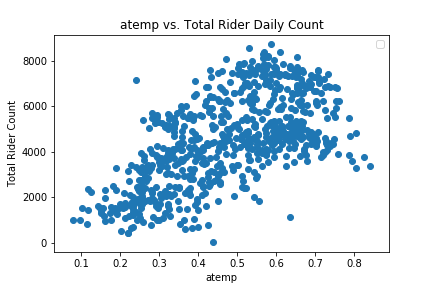
\includegraphics[width=50mm]{Bike-Sharing-Dataset/images/day_atemp.png}
\end{subfigure}
\begin{subfigure} 
    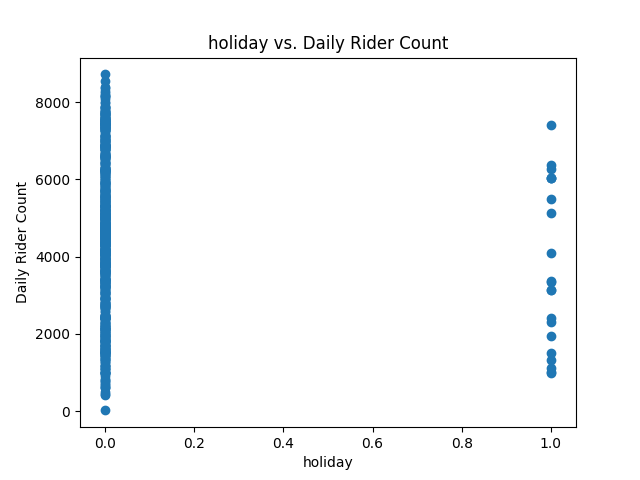
\includegraphics[width=50mm]{Bike-Sharing-Dataset/images/day_holiday.png}
\end{subfigure}
\begin{subfigure} 
    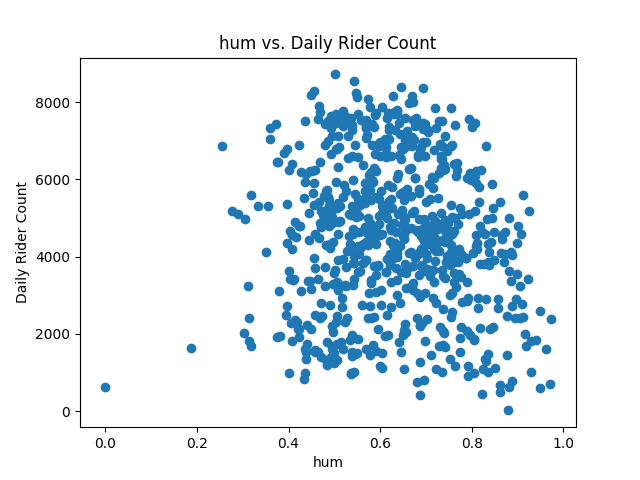
\includegraphics[width=50mm]{Bike-Sharing-Dataset/images/day_hum.png}
\end{subfigure}
\begin{subfigure} 
    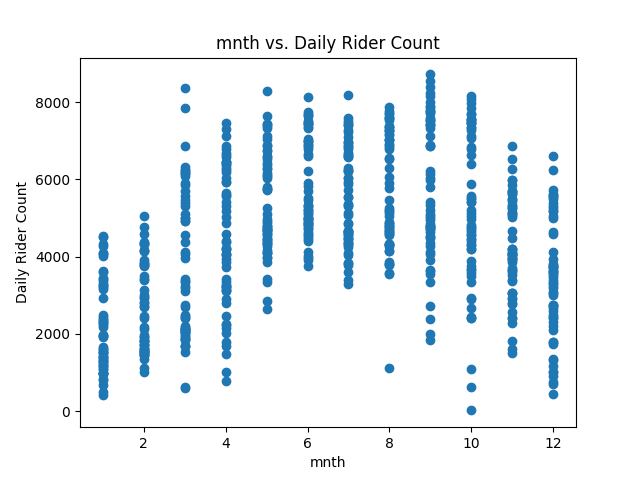
\includegraphics[width=50mm]{Bike-Sharing-Dataset/images/day_mnth.png}
\end{subfigure}
\begin{subfigure} 
    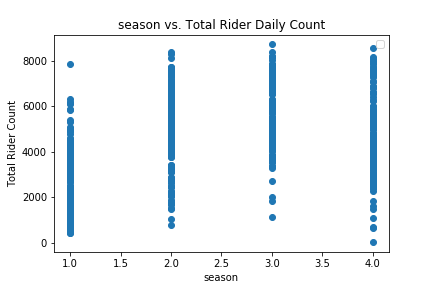
\includegraphics[width=50mm]{Bike-Sharing-Dataset/images/day_season.png}
\end{subfigure}
\begin{subfigure} 
    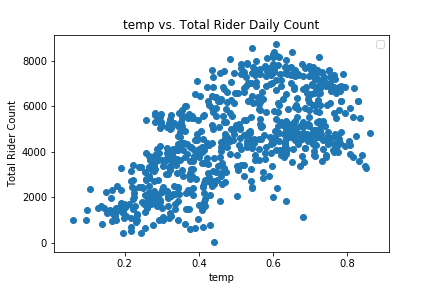
\includegraphics[width=50mm]{Bike-Sharing-Dataset/images/day_temp.png}
\end{subfigure}
\begin{subfigure} 
    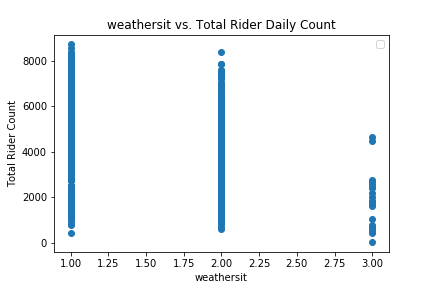
\includegraphics[width=50mm]{Bike-Sharing-Dataset/images/day_weathersit.png}
\end{subfigure}
\begin{subfigure} 
    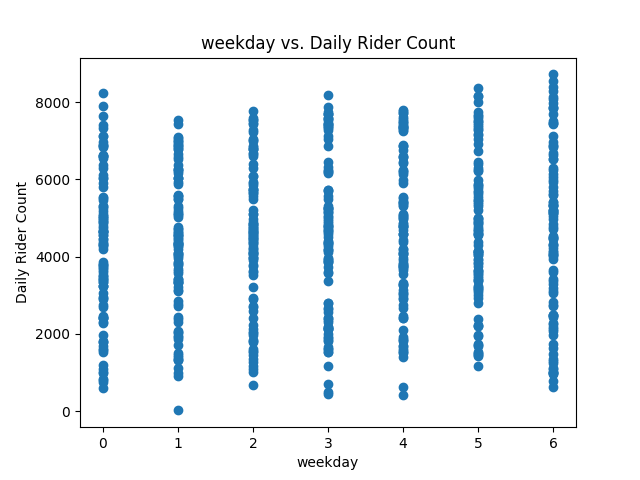
\includegraphics[width=50mm]{Bike-Sharing-Dataset/images/day_weekday.png}
\end{subfigure}
\begin{subfigure} 
    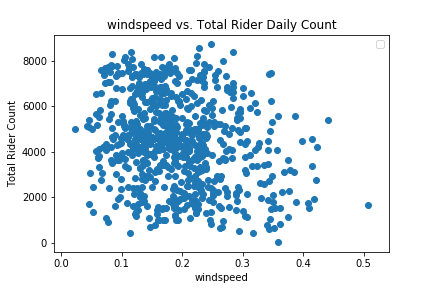
\includegraphics[width=50mm]{Bike-Sharing-Dataset/images/day_windspeed.png}
\end{subfigure}
\begin{subfigure} 
    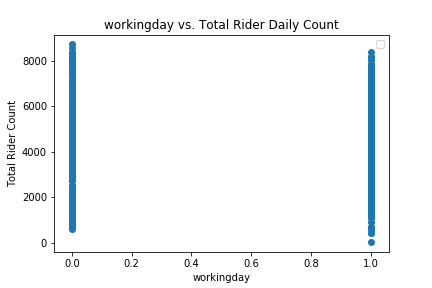
\includegraphics[width=50mm]{Bike-Sharing-Dataset/images/day_workingday.png}
\end{subfigure}
\begin{subfigure} 
    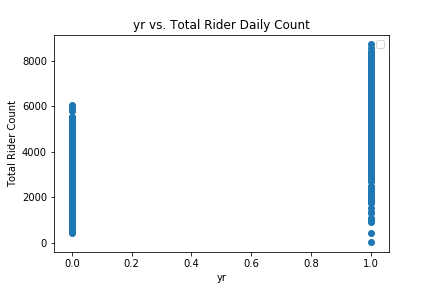
\includegraphics[width=50mm]{Bike-Sharing-Dataset/images/day_yr.png}
\end{subfigure}
\end{figure}

\newpage
\begin{figure}[h]
\centering
\begin{subfigure} 
    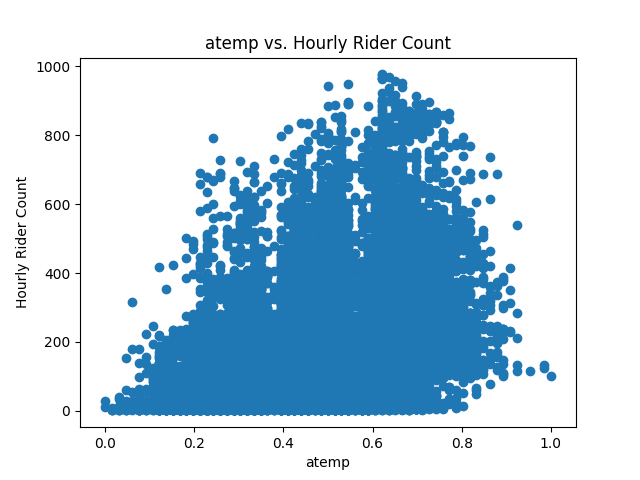
\includegraphics[width=50mm]{Bike-Sharing-Dataset/images/hour_atemp.png}
\end{subfigure}
\begin{subfigure} 
    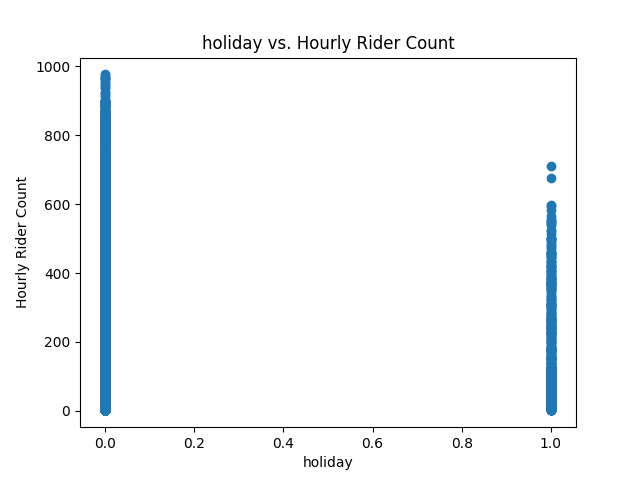
\includegraphics[width=50mm]{Bike-Sharing-Dataset/images/hour_holiday.png}
\end{subfigure}
\begin{subfigure} 
    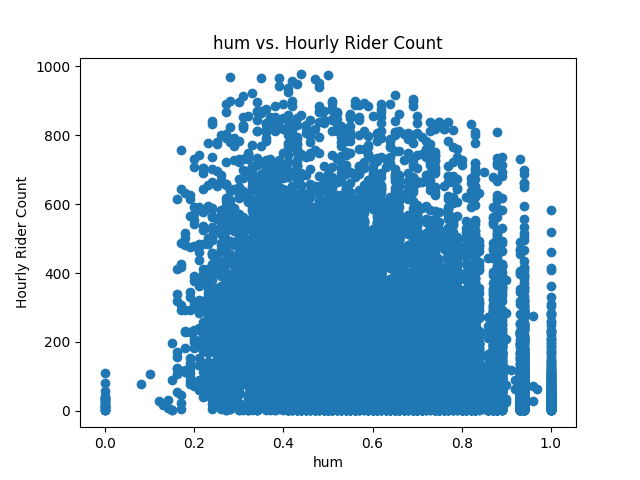
\includegraphics[width=50mm]{Bike-Sharing-Dataset/images/hour_hum.png}
\end{subfigure}
\begin{subfigure} 
    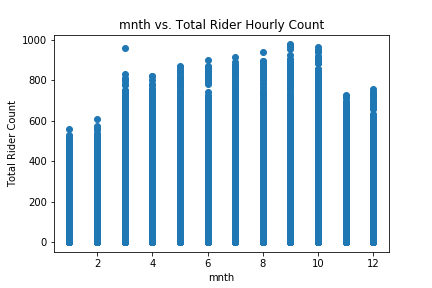
\includegraphics[width=50mm]{Bike-Sharing-Dataset/images/hour_mnth.png}
\end{subfigure}
\begin{subfigure} 
    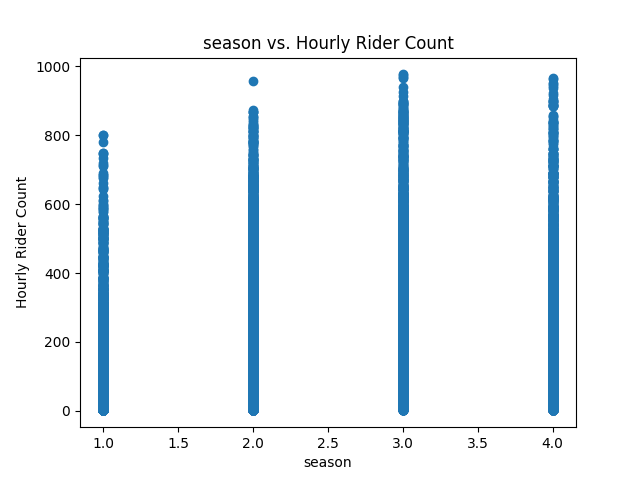
\includegraphics[width=50mm]{Bike-Sharing-Dataset/images/hour_season.png}
\end{subfigure}
\begin{subfigure} 
    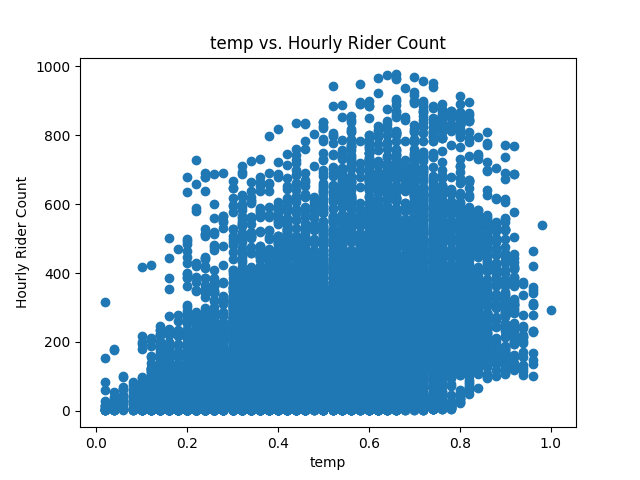
\includegraphics[width=50mm]{Bike-Sharing-Dataset/images/hour_temp.png}
\end{subfigure}
\begin{subfigure} 
    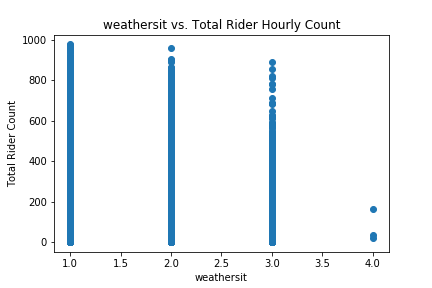
\includegraphics[width=50mm]{Bike-Sharing-Dataset/images/hour_weathersit.png}
\end{subfigure}
\begin{subfigure} 
    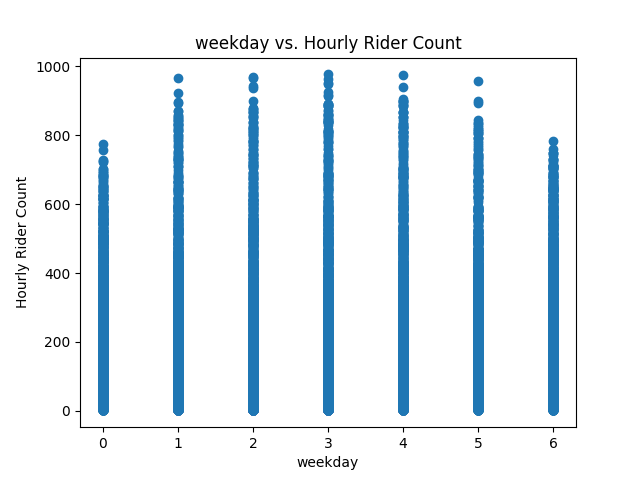
\includegraphics[width=50mm]{Bike-Sharing-Dataset/images/hour_weekday.png}
\end{subfigure}
\begin{subfigure} 
    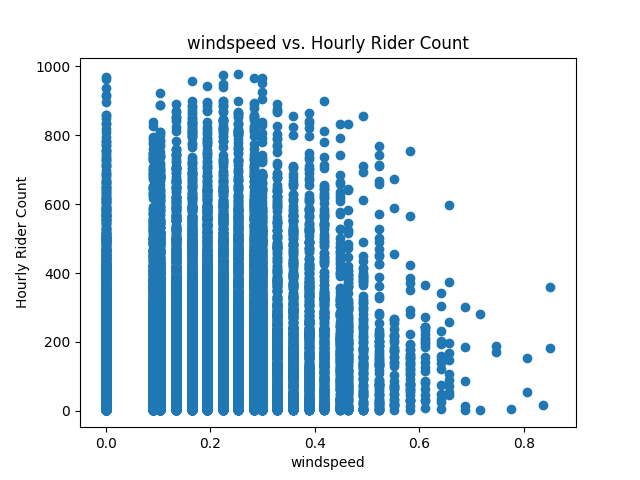
\includegraphics[width=50mm]{Bike-Sharing-Dataset/images/hour_windspeed.png}
\end{subfigure}
\begin{subfigure} 
    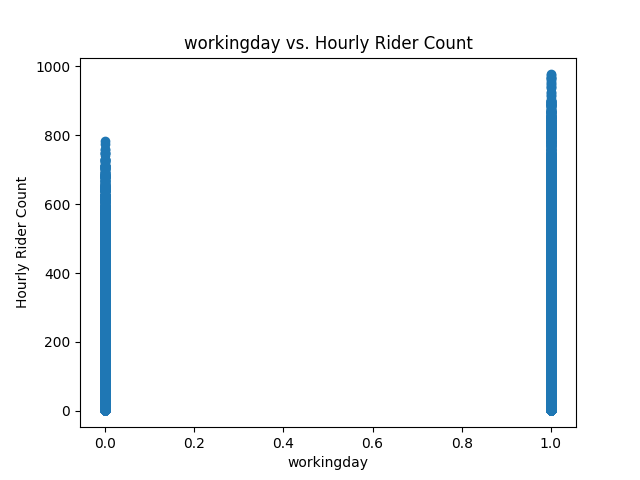
\includegraphics[width=50mm]{Bike-Sharing-Dataset/images/hour_workingday.png}
\end{subfigure}
\begin{subfigure} 
    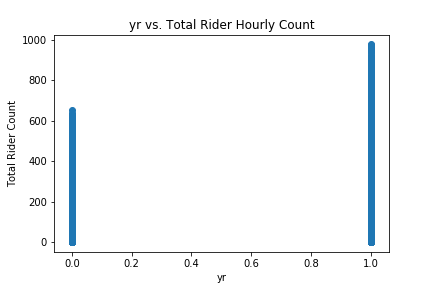
\includegraphics[width=50mm]{Bike-Sharing-Dataset/images/hour_yr.png}
\end{subfigure}
\end{figure}

\newpage
Based on the feature graphs, temperature was reduced to the best feature to model. According to the \texttt{README} the temperature was normalized with a \SI{41}{\celsius} maximum so the temperature array is multiplied by 41 for human readability. 

\begin{lstlisting}[language=Python, firstnumber=37]
day_temp = day["temp"].values.reshape(-1, 1) * 41
\end{lstlisting}

KFold cross-validation was used with a 10-split. The regression models applied were linear, ridge, lasso, and bayesian through their respective \texttt{sklearn} packages. For each k-fold, the models are fitted using the separated training data. 

\begin{lstlisting}[language=Python, firstnumber=39]
crossvalidation = KFold(n_splits=10)
linear = LinearRegression()
ridge = Ridge()
lasso = Lasso()
bayesian = BayesianRidge()

for train_index, test_index in crossvalidation.split(day_temp):
    X_train, X_test = day_temp[train_index], day_temp[test_index]
    y_train, y_test = cnt_day[train_index], cnt_day[test_index]
    linear.fit(X_train, y_train)
    ridge.fit(X_train, y_train)
    lasso.fit(X_train, y_train)
\end{lstlisting}

The test portion of the data was then used to test the prediction quality of the models. The mean square error was calculated between the test portion data and the values predicted by the models. 

\begin{lstlisting}[language=Python, firstnumber=53]
linear_pred = linear.predict(X_test)
ridge_pred = ridge.predict(X_test)
lasso_pred = lasso.predict(X_test)
bayesian_pred = bayesian.predict(X_test)

mse_linear = mean_squared_error(y_test, linear_pred)
mse_ridge = mean_squared_error(y_test, ridge_pred)
mse_lasso = mean_squared_error(y_test, lasso_pred)
mse_bayesian = mean_squared_error(y_test, bayesian_pred)
\end{lstlisting}

The following a table showing the different mean squared error values of the models. 

\begin{table}[h]
    \centering
    \begin{tabular}{|l|l|}
    \hline
    Model  & Mean Squared Error \\ \hline
    Linear & 4306257.419012716 \\ 
    Ridge  & 4306194.805960745 \\ 
    Lasso  & 4306018.563140404 \\ 
    Bayesian & 4301889.80709847 \\
    \hline
    \end{tabular}
\end{table}

\newpage
\begin{figure}[h]
    \centering
    \begin{subfigure} 
        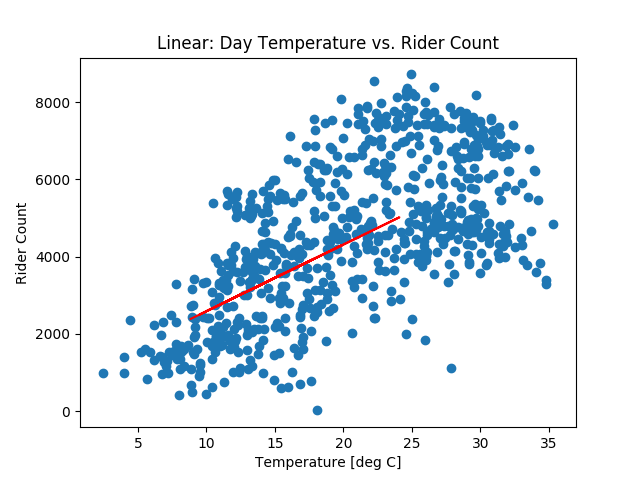
\includegraphics[width=75mm]{Bike-Sharing-Dataset/images/linear.png}
    \end{subfigure}
    \begin{subfigure} 
        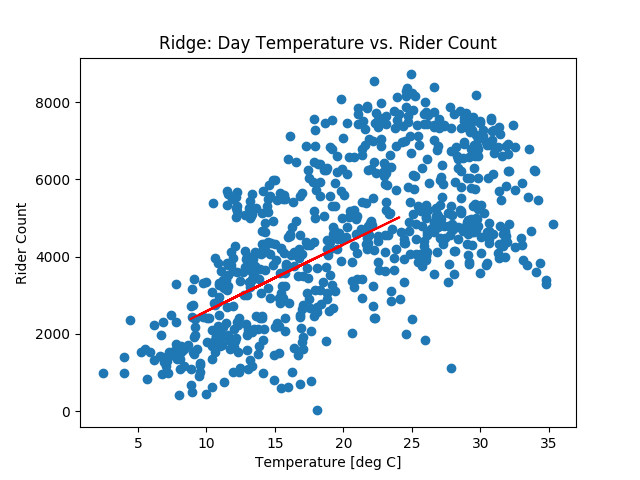
\includegraphics[width=75mm]{Bike-Sharing-Dataset/images/ridge.png}
    \end{subfigure}
    \begin{subfigure} 
        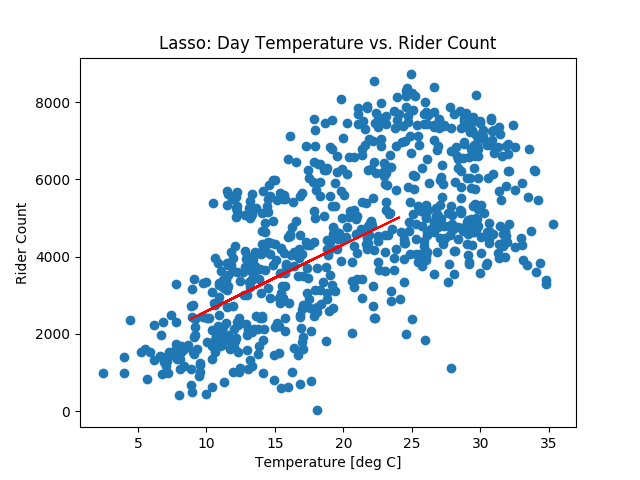
\includegraphics[width=75mm]{Bike-Sharing-Dataset/images/lasso.png}
    \end{subfigure}
    \begin{subfigure} 
        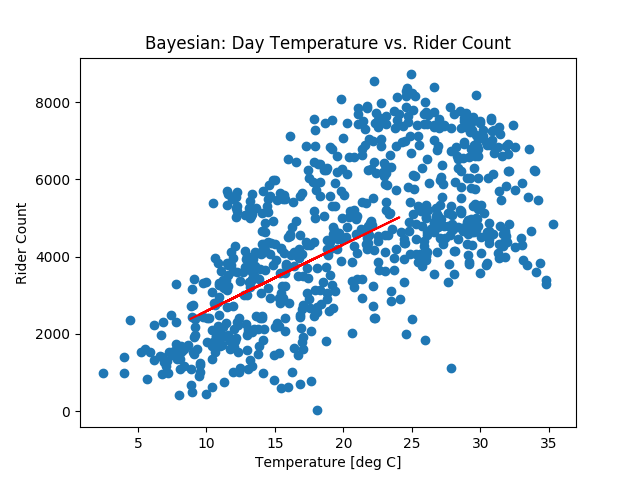
\includegraphics[width=75mm]{Bike-Sharing-Dataset/images/bayesian.png}
    \end{subfigure}
    \end{figure}

\end{solution}

\newpage
\begin{problem}[5]
    UCI Machine Learning: Iris Data Set 
    
    \begin{enumerate}[label=\alph*.]
        \item Implement Linear Discriminant Analysis for each pair of the classes and report your results. Note that there are three class labels in the data set. Write down each step of your solution.  
 
        \item Perform the kNN classification for each k value from 1 to 50 to predict the species. For each k value, compute the percentage of misclassified values on the testing set. Print out your results as a table showing the values of k and the misclassification percentages. Then plot the misclassification rates on the testing set versus the k values. 
    \end{enumerate}
\end{problem}

\begin{solution}

\begin{enumerate}[label=\alph*.]
    \item The necessary packages and data were imported. 

\begin{lstlisting}[language=Python]
import matplotlib.pyplot as plt

from sklearn import datasets
from sklearn.discriminant_analysis import LinearDiscriminantAnalysis as LDA

iris = datasets.load_iris()

X = iris.data
y = iris.target
names = iris.target_names
\end{lstlisting}

The linear discriminant analysis function from the Sklearn package was used to implement the analysis.  

\begin{lstlisting}[language=Python, firstnumber=12]
lda = LDA(n_components=2)
model = lda.fit(X, y).transform(X)

plt.figure()
for i, name in zip([0, 1, 2], names):
    plt.scatter(model[y == i, 0], model[y == i, 1], label=name)
plt.legend()
plt.xlabel("LD1")
plt.ylabel("LD2")
plt.show()
\end{lstlisting}

\begin{figure}[h]
    \centering
    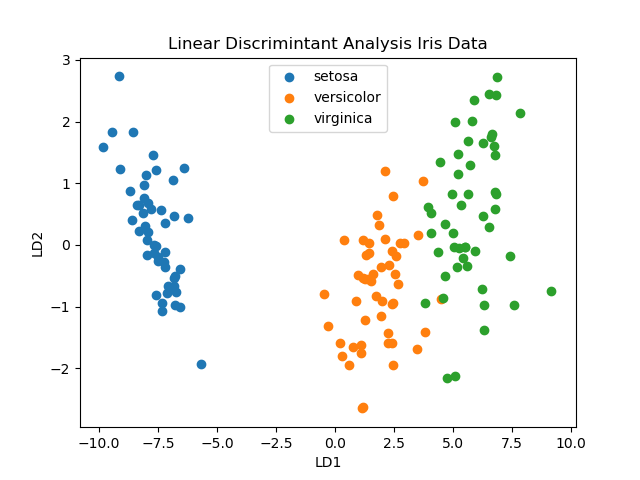
\includegraphics[width=75mm]{Iris/LDA.png}
\end{figure}

\newpage
\item The data was split to accommodate for a 20\% testing set. For each iteration of K (from 1 to 50) a k-nearest neighbor classifier model is generated with the training data and then tested using the testing set. The accuracy score is calculated and stored. I encountered a problem where there was an inconsistent score given every time I ran the script. 

\begin{lstlisting}[language=Python, firstnumber=14]
X_train, X_test, y_train, y_test = train_test_split(X, y, test_size=0.2)

k_range = range(1,51)

scores = {}
scores_list = []
print("K Value | Accuracy Score")
for k in k_range:
    knn = KNeighborsClassifier(n_neighbors=k)
    knn.fit(X_train, y_train)
    pred = knn.predict(X_test)
    scores[k] = metrics.accuracy_score(y_test, pred)
    scores_list.append(scores[k])
    print("%i | %f"%(k, scores[k]))

plt.figure()
plt.plot(k_range, scores_list)
plt.title("Misclassification Rate")
plt.xlabel("KNN K Value")
plt.ylabel("Accuracy")
plt.show()

\end{lstlisting}

\begin{table}[h]
    \centering
    \resizebox{\textwidth}{!}{%
    \begin{tabular}{l|ll|ll|ll|ll|l}
        K Value & Accuracy Score & \multicolumn{8}{l}{}                                          \\
       \hline \\
    1  & 0.966667 & 11 & 0.966667 & 21 & 0.966667 & 31 & 0.966667 & 41 & 0.966667 \\
    2  & 0.933333 & 12 & 0.966667 & 22 & 0.966667 & 32 & 0.966667 & 42 & 0.933333 \\
    3  & 0.966667 & 13 & 0.966667 & 23 & 0.966667 & 33 & 0.966667 & 43 & 0.966667 \\
    4  & 0.966667 & 14 & 0.966667 & 24 & 0.966667 & 34 & 0.966667 & 44 & 0.933333 \\
    5  & 0.966667 & 15 & 0.966667 & 25 & 0.966667 & 35 & 0.966667 & 45 & 0.933333 \\
    6  & 0.933333 & 16 & 0.966667 & 26 & 0.966667 & 36 & 0.966667 & 46 & 0.933333 \\
    7  & 0.933333 & 17 & 0.966667 & 27 & 0.966667 & 37 & 0.966667 & 47 & 0.966667 \\
    8  & 0.966667 & 18 & 0.966667 & 28 & 0.966667 & 38 & 0.933333 & 48 & 0.933333 \\
    9  & 0.966667 & 19 & 0.966667 & 29 & 0.966667 & 39 & 0.966667 & 49 & 0.966667 \\
    10 & 0.966667 & 20 & 0.966667 & 30 & 0.966667 & 40 & 0.933333 & 50 & 0.933333
    \end{tabular}
    }
\end{table}

\begin{figure}[h]
    \centering
    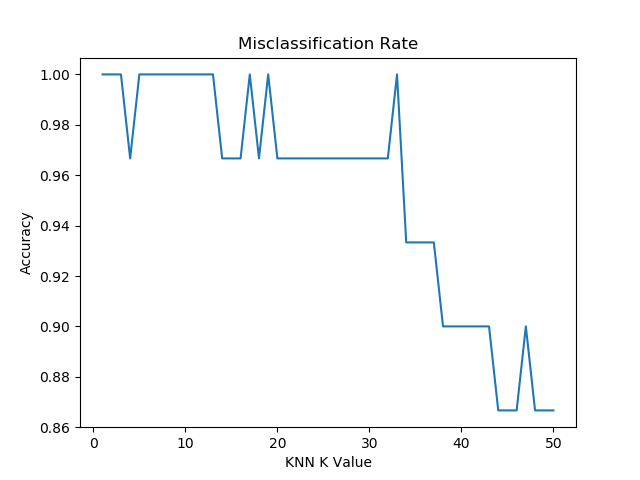
\includegraphics[width=75mm]{Iris/knn.png}
\end{figure}

\end{enumerate}
\end{solution}

\end{document}